\section{Contribution}

\subsection{Statistics Extraction}

\begin{frame}[shrink=10] %hmm.. thought i could change colour here :S
\frametitle{Statistics Extraction} 


    \begin{tabular}{ccc}
\begin{tabular}{@{}|c@{}|c@{}|@{}}
\hline
Timestamp & Query \\ \hline 
$T_1$ & $Q_{3,6}$ \\ \hline 
$T_2$ & $Q_{1,6}$ \\ \hline 
$T_3$ & $Q_{2,7}$ \\ \hline 
$T_4$ & $Q_{1,4}$ \\ \hline 
$T_5$ & $Q_{4,8}$ \\ \hline 
$T_6$ & $Q_{2,5}$ \\ \hline 
$T_7$ & $Q_{3,6}$ \\ \hline  
$T_8$ & $Q_{3,6}$ \\ \hline 
\end{tabular}
&
    \begin{tabular}{|@{ }c@{ }|@{ }c@{ }c@{ }c@{ }c@{ }c@{ }c@{ }c@{ }c@{ }|}
       \hline
       $\chi_{s,t}$	& $v_1$	& $v_2$	& $v_3$	& $v_4$	& $v_5$	& $v_6$	& $v_7$ & $v_8$ \\\hline
       $v_1$			& /	& 0	& 0	& 1	& 0	& 1	& 0	& 0	 \\
       $v_2$			& 0	& /	& 0	& 0	& 1	& 0	& 1	& 0	 \\
       $v_3$			& 0	& 0	& /	& 0	& 0	& 3	& 0	& 0	 \\
       $v_4$			& 1	& 0	& 0	& /	& 0	& 0	& 0	& 1	 \\
       $v_5$			& 0	& 1	& 0	& 0	& /	& 0	& 0	& 0	 \\
       $v_6$			& 1	& 0	& 3	& 0	& 0	& /	& 0	& 0	 \\
       $v_7$			& 0	& 1	& 0	& 0	& 0	& 0	& / & 0  \\
       $v_8$			& 0	& 0	& 0	& 1	& 0	& 0	& 0 & /  \\
       \hline
    \end{tabular}
	\\
    \end{tabular}\\

\hspace{10em}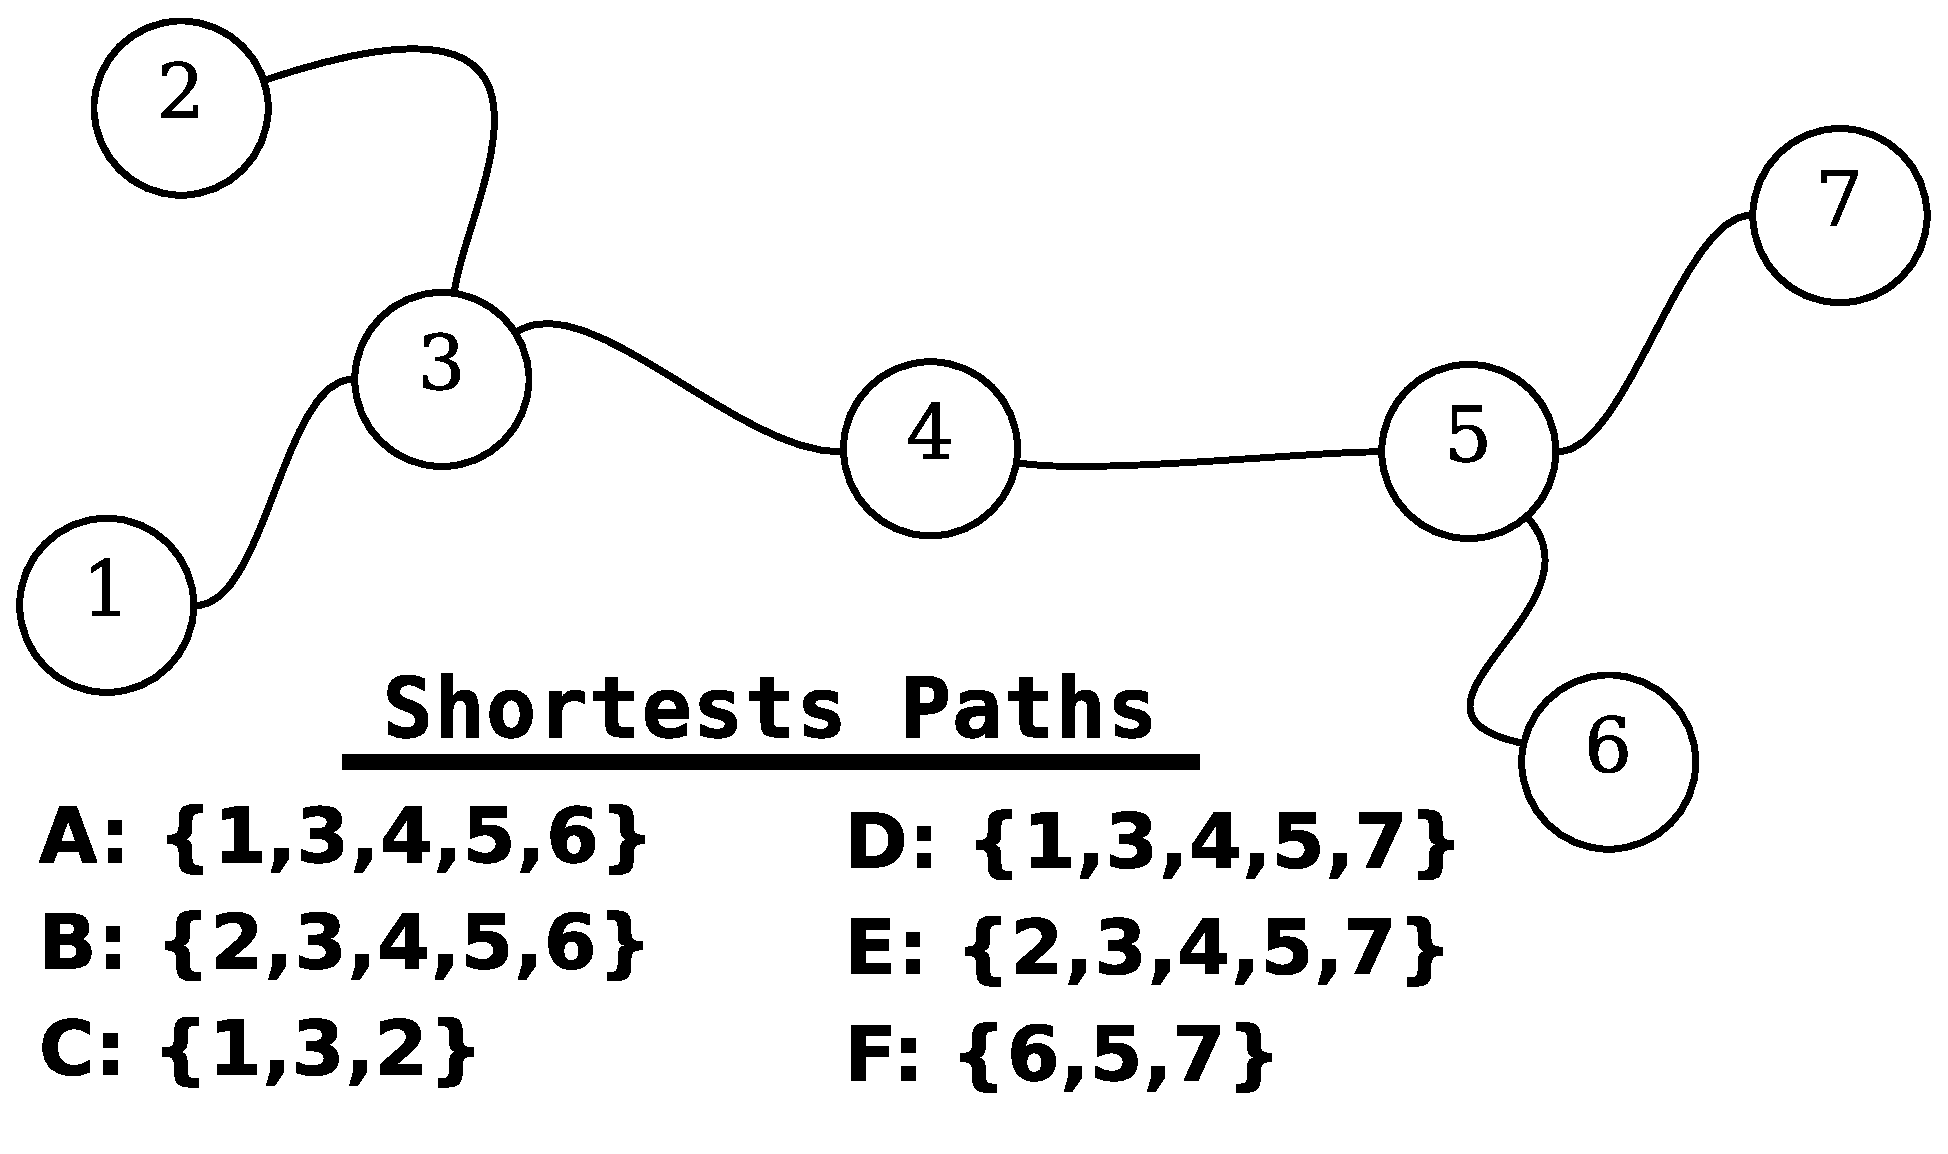
\includegraphics[width=0.55\columnwidth]{images/rxmap} 


\end{frame}

\begin{frame}[shrink=10] %hmm.. thought i could change colour here :S
\frametitle{Grouping} 

\begin{tabular}{lc}

    \begin{tabular}{|@{ }c@{ }|@{ }c@{ }c@{ }c@{ }c@{ }c@{ }c@{ }c@{ }c@{ }|}
       \hline
       $\chi_{s,t}$	& $v_1$	& $v_2$	& $v_3$	& $v_4$	& $v_5$	& $v_6$	& $v_7$ & $v_8$ \\\hline
       $v_1$			& /	& 0	& 0	& 1	& 0	& 1	& 0	& 0	 \\
       $v_2$			& 0	& /	& 0	& 0	& 1	& 0	& 1	& 0	 \\
       $v_3$			& 0	& 0	& /	& 0	& 0	& 3	& 0	& 0	 \\
       $v_4$			& 1	& 0	& 0	& /	& 0	& 0	& 0	& 1	 \\
       $v_5$			& 0	& 1	& 0	& 0	& /	& 0	& 0	& 0	 \\
       $v_6$			& 1	& 0	& 3	& 0	& 0	& /	& 0	& 0	 \\
       $v_7$			& 0	& 1	& 0	& 0	& 0	& 0	& / & 0  \\
       $v_8$			& 0	& 0	& 0	& 1	& 0	& 0	& 0 & /  \\
       \hline
    \end{tabular}
&
\multirow{3}{*}{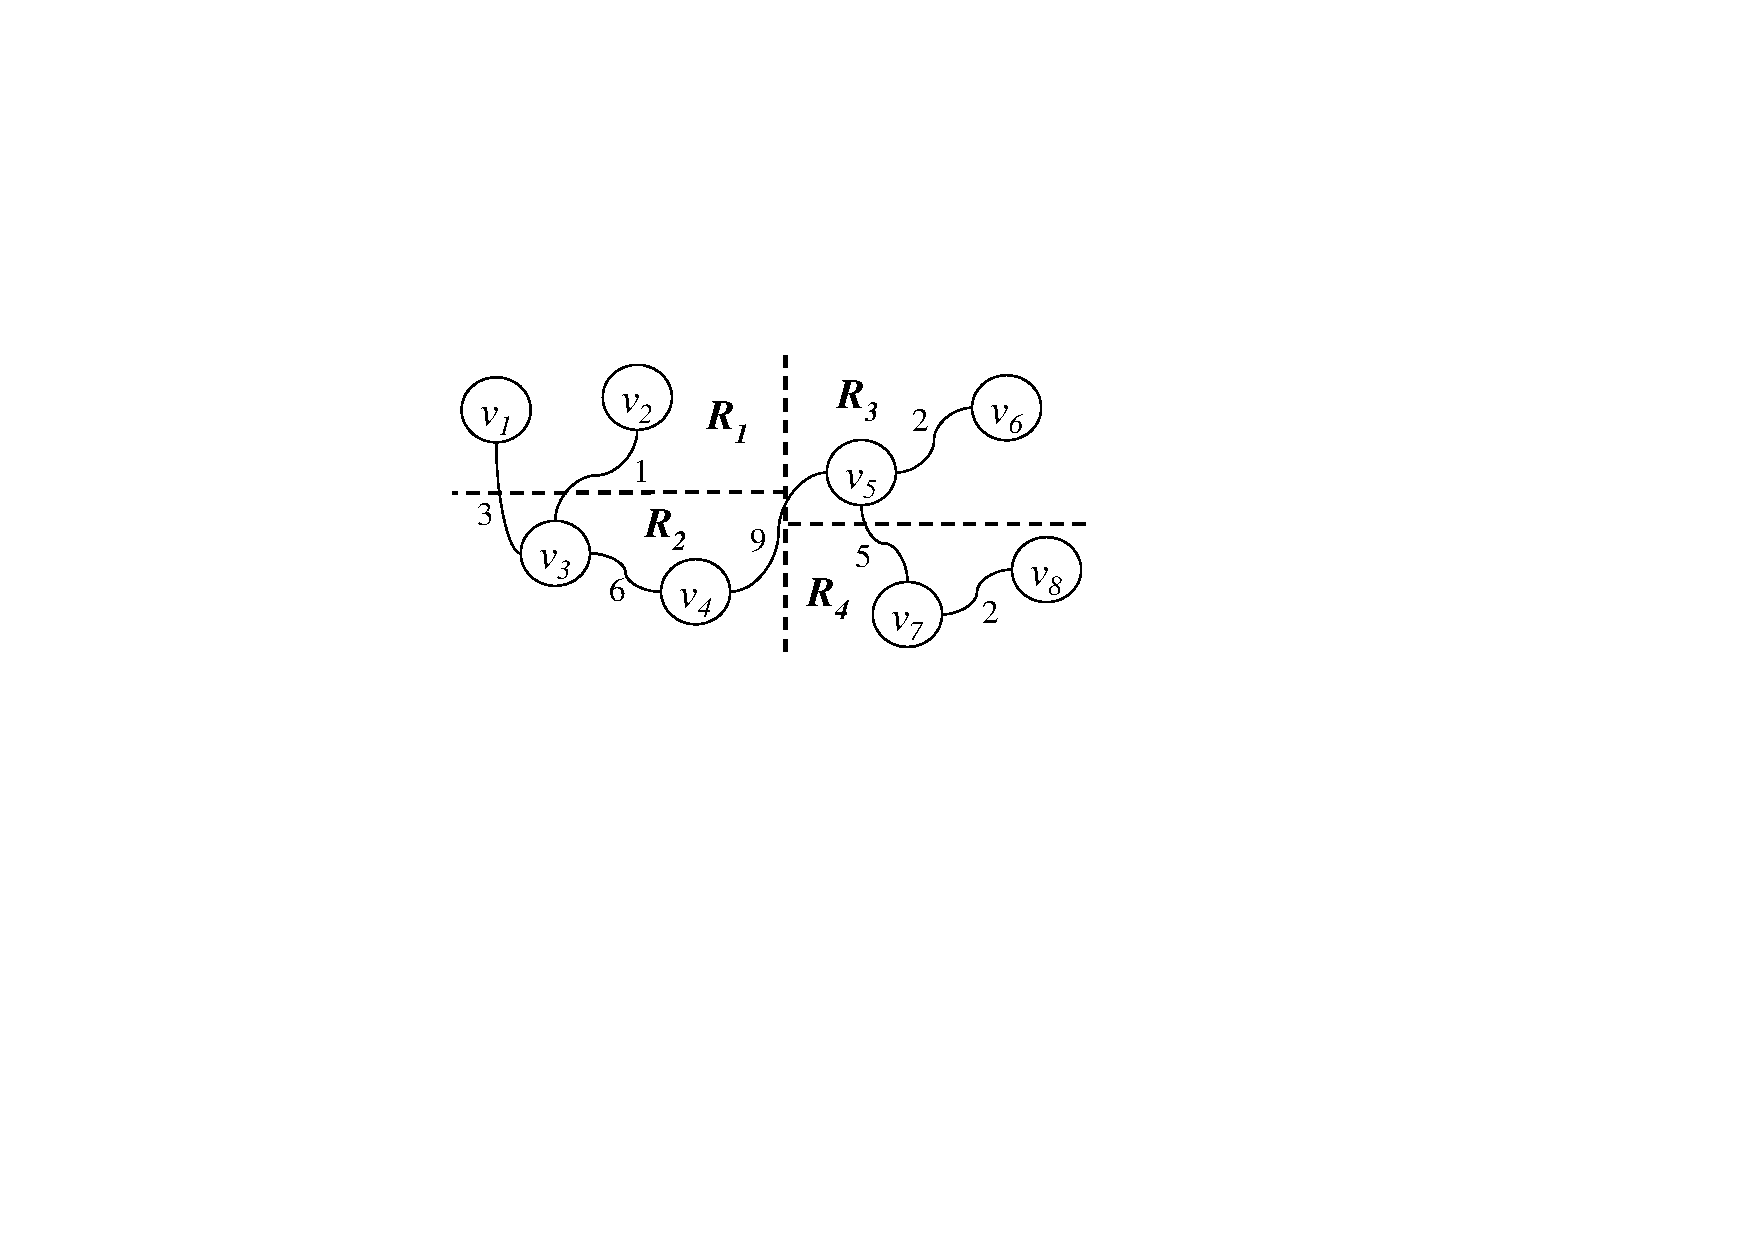
\includegraphics[width=0.68\columnwidth]{images/mappartition}} \\
& \\

	\begin{tabular}{|@{ }c@{ }|@{ }c@{ }c@{ }c@{ }c@{ }|}
	\hline \small
	\textbf{$\chi_{R_i,R_j}$}	& $R_1$		& $R_2$		& $R_3$		& $R_4$\\\hline
	$R_1$			& 0	& 1	& 2	& 1 \\ 
	$R_2$			& 1	& 0	& 3	& 1 \\ 
	$R_3$			& 2	& 3	& 0	& 0 \\ 
	$R_4$			& 1	& 1	& 0	& 0 \\ 
	\hline
	\end{tabular}
	\\
&
% \multicolumn{2}{c}{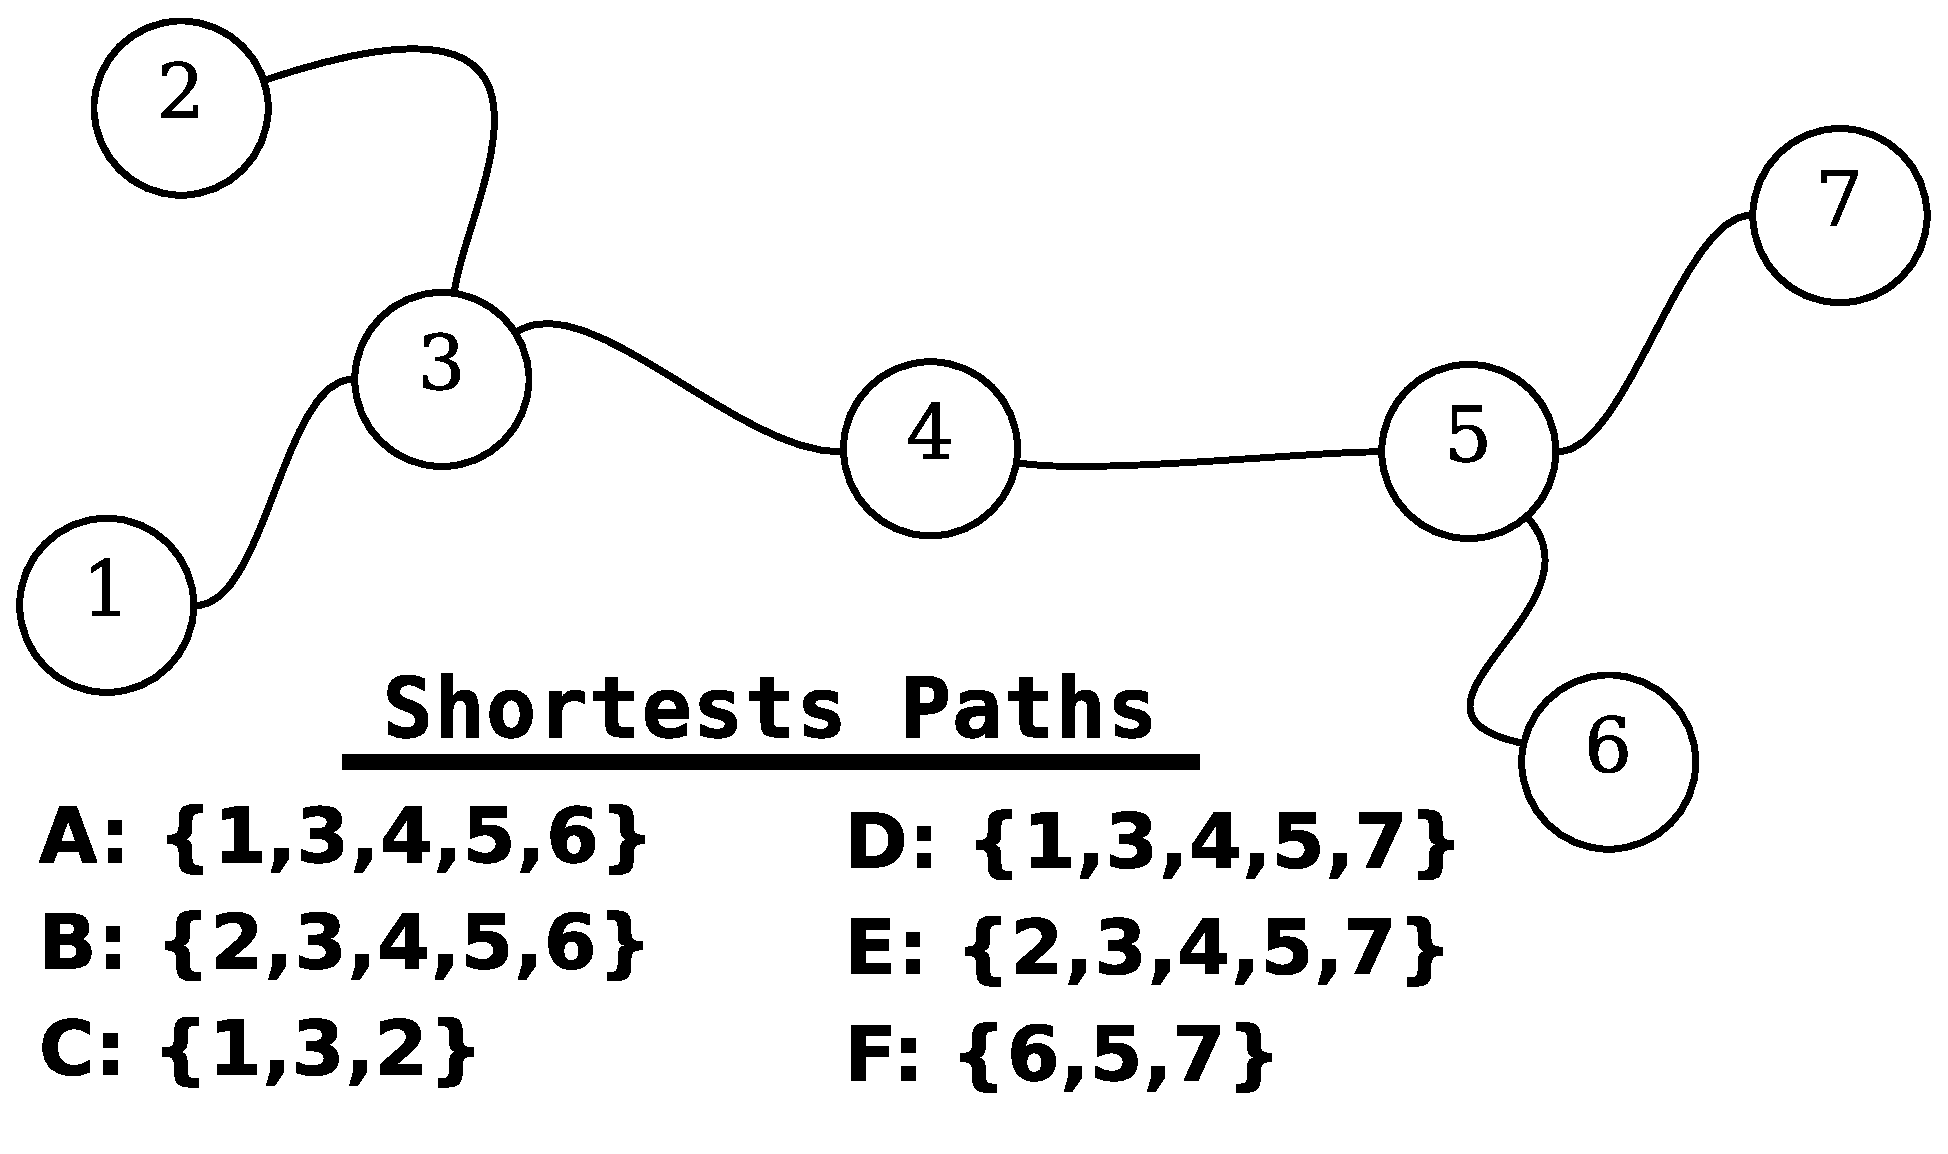
\includegraphics[width=0.75\columnwidth]{images/rxmap}}
  
\end{tabular}

\end{frame}



\subsection{Cost Estimation}
\begin{frame}[red] %hmm.. thought i could change colour here :S
\frametitle{SP Call Cost Estimation} 


\begin{columns}[b]
  \begin{column}{0.5\textwidth}
\begin{exampleblock}{Proxy Scenario}
$E_{s,t}(Proxy) = 1$
\end{exampleblock}

\begin{exampleblock}{Server Scenario}
Intuition: Longer query results incur higher cost.
\end{exampleblock}

$-$ Cost only estimated in server scenario\\
$-$ Estimation methods developed for Server scenario
  \end{column}
  \begin{column}{0.45\textwidth}

  \end{column}
\end{columns}


  \begin{picture}(0.0,0.0) 
     \put(160,30){  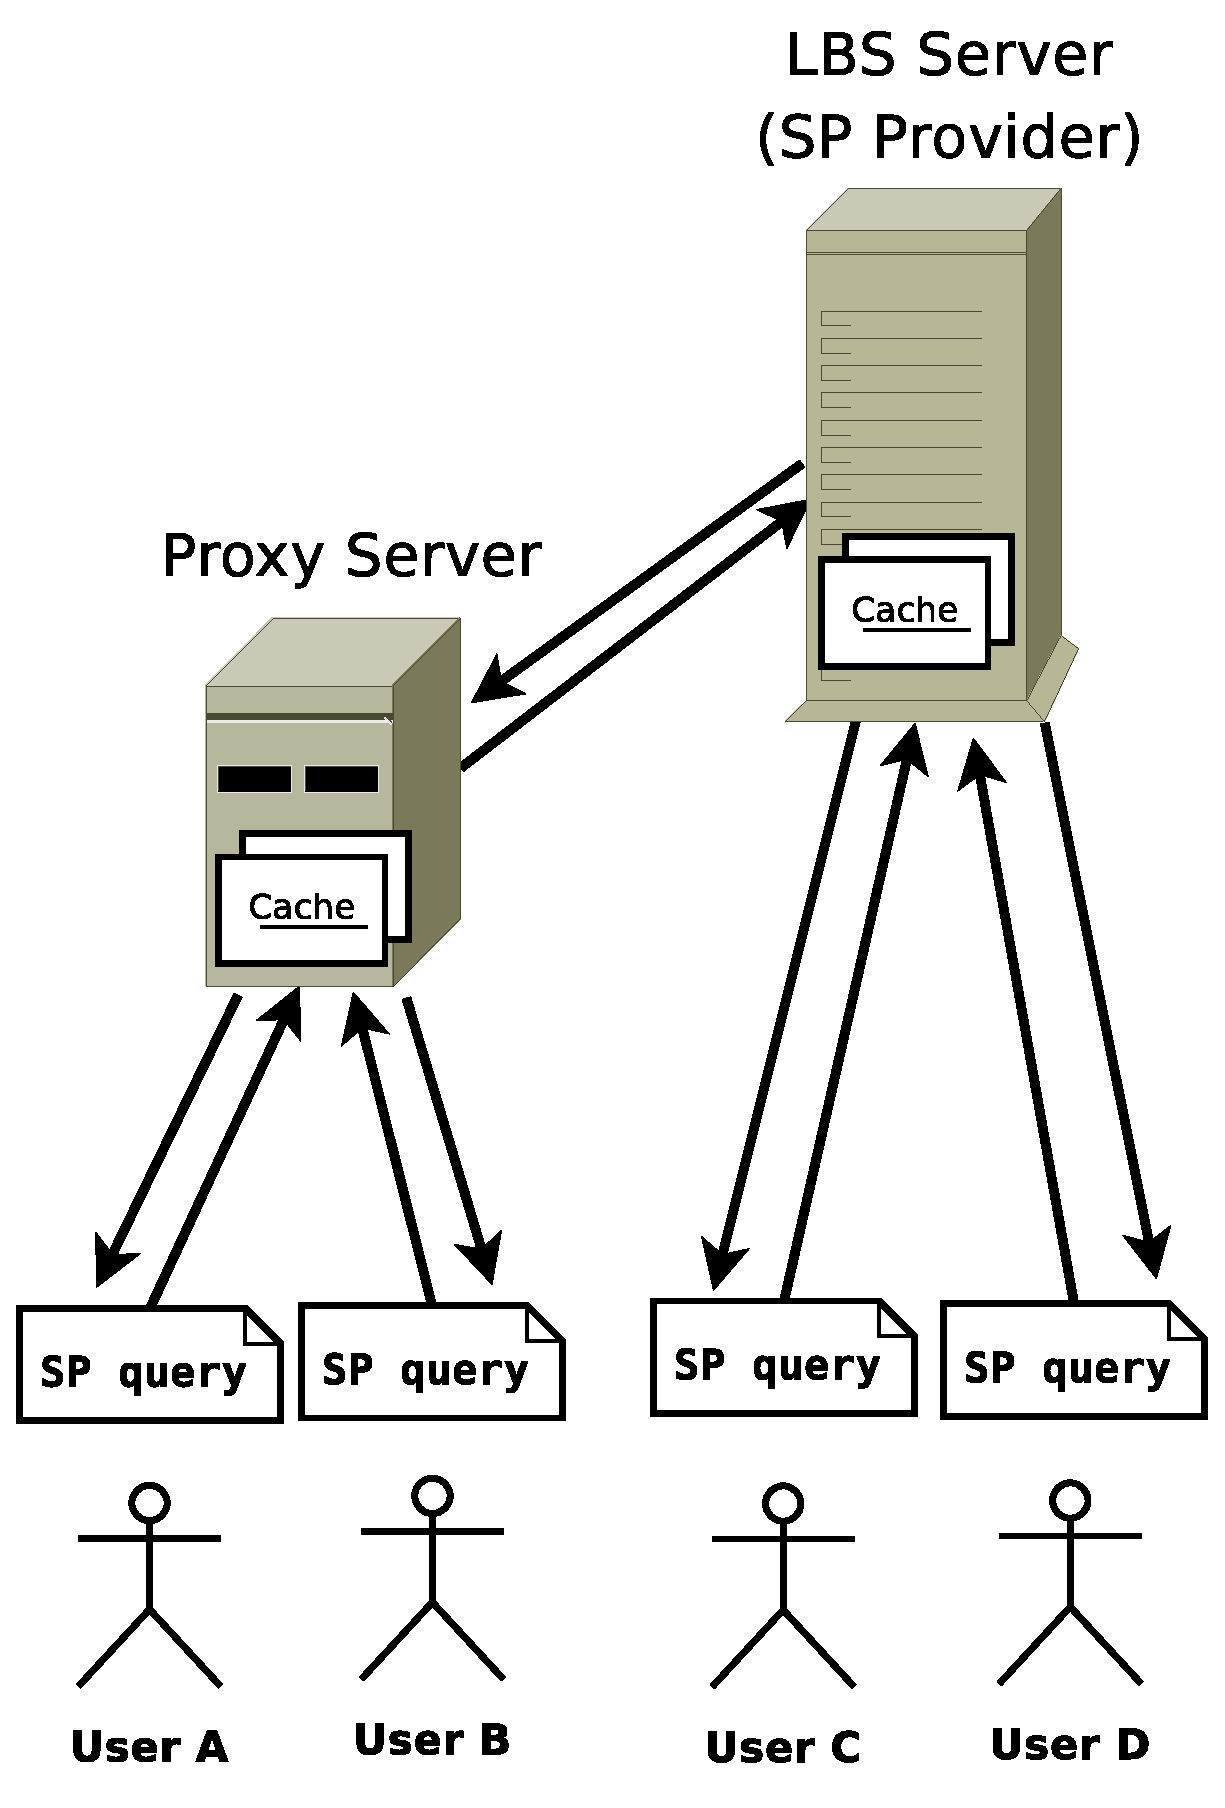
\includegraphics[width=0.5\textwidth]{images/scenario} }
  \end{picture}



% Two data structures:
% \begin{itemize}
%   \item Distance estimator, Landmark-based [Potamias et al. CIKM]
%   \item Expense histogram
% \end{itemize}
\end{frame}


\subsection{Benefit Model}



\begin{frame} %hmm.. thought i could change colour here :S
\frametitle{Incremental Benefit per size} 
  \begin{block}{Benefit formula}
    $\Delta\overline{\gamma}(P_{a,b}, \Psi) = \sum\limits_{P_{s,t} \in \mathfrak{U}(P_{a,b}) - \mathfrak{U}(\Psi)} \frac{\chi_{s,t} * E_{s,t}}{|P_{a,b}|}$
  \end{block}


\begin{itemize}
\item $P_{a,b}$: a shortest path 
\item $\Psi$: the cache 
\item $\mathfrak{U}(P_{a,b})$: all sub-paths of $P_{a,b}$. 
\item $\chi_{s,t}$ frequency of query $s$ to $t$. 
\item $E_{s,t}$: cost of calculating $P_{s,t}$
\end{itemize}

\end{frame}

% \begin{frame} %hmm.. thought i could change colour here :S
% % \frametitle{Benefit Model} 
% 
% \begin{columns}
%   \begin{column}{0.4\textwidth}
% From Query Log:
%   \begin{tabular}{|l|l|}
%     Shortest Path & Frequency \\\hline
%     $P_{3,6}$ & 3 \\
%     $P_{1,4}$ & 1 \\
%     $P_{1,6}$ & 1 \\
%   \end{tabular}
%   \end{column}
%   \begin{column}{0.1\textwidth}
%   \end{column}
%   \begin{column}[t]{0.6\textwidth}
% Cost Estimation:\\
%   \begin{tabular}{|l|l|}
%     Shortest Path & Cost \\\hline
%     $P_{3,6}$ & 3 \\
%     $P_{1,4}$ & 2 \\
%     $P_{1,6}$ & 4 \\
%   \end{tabular}
%   \end{column}
% \end{columns}
% 
% 
%     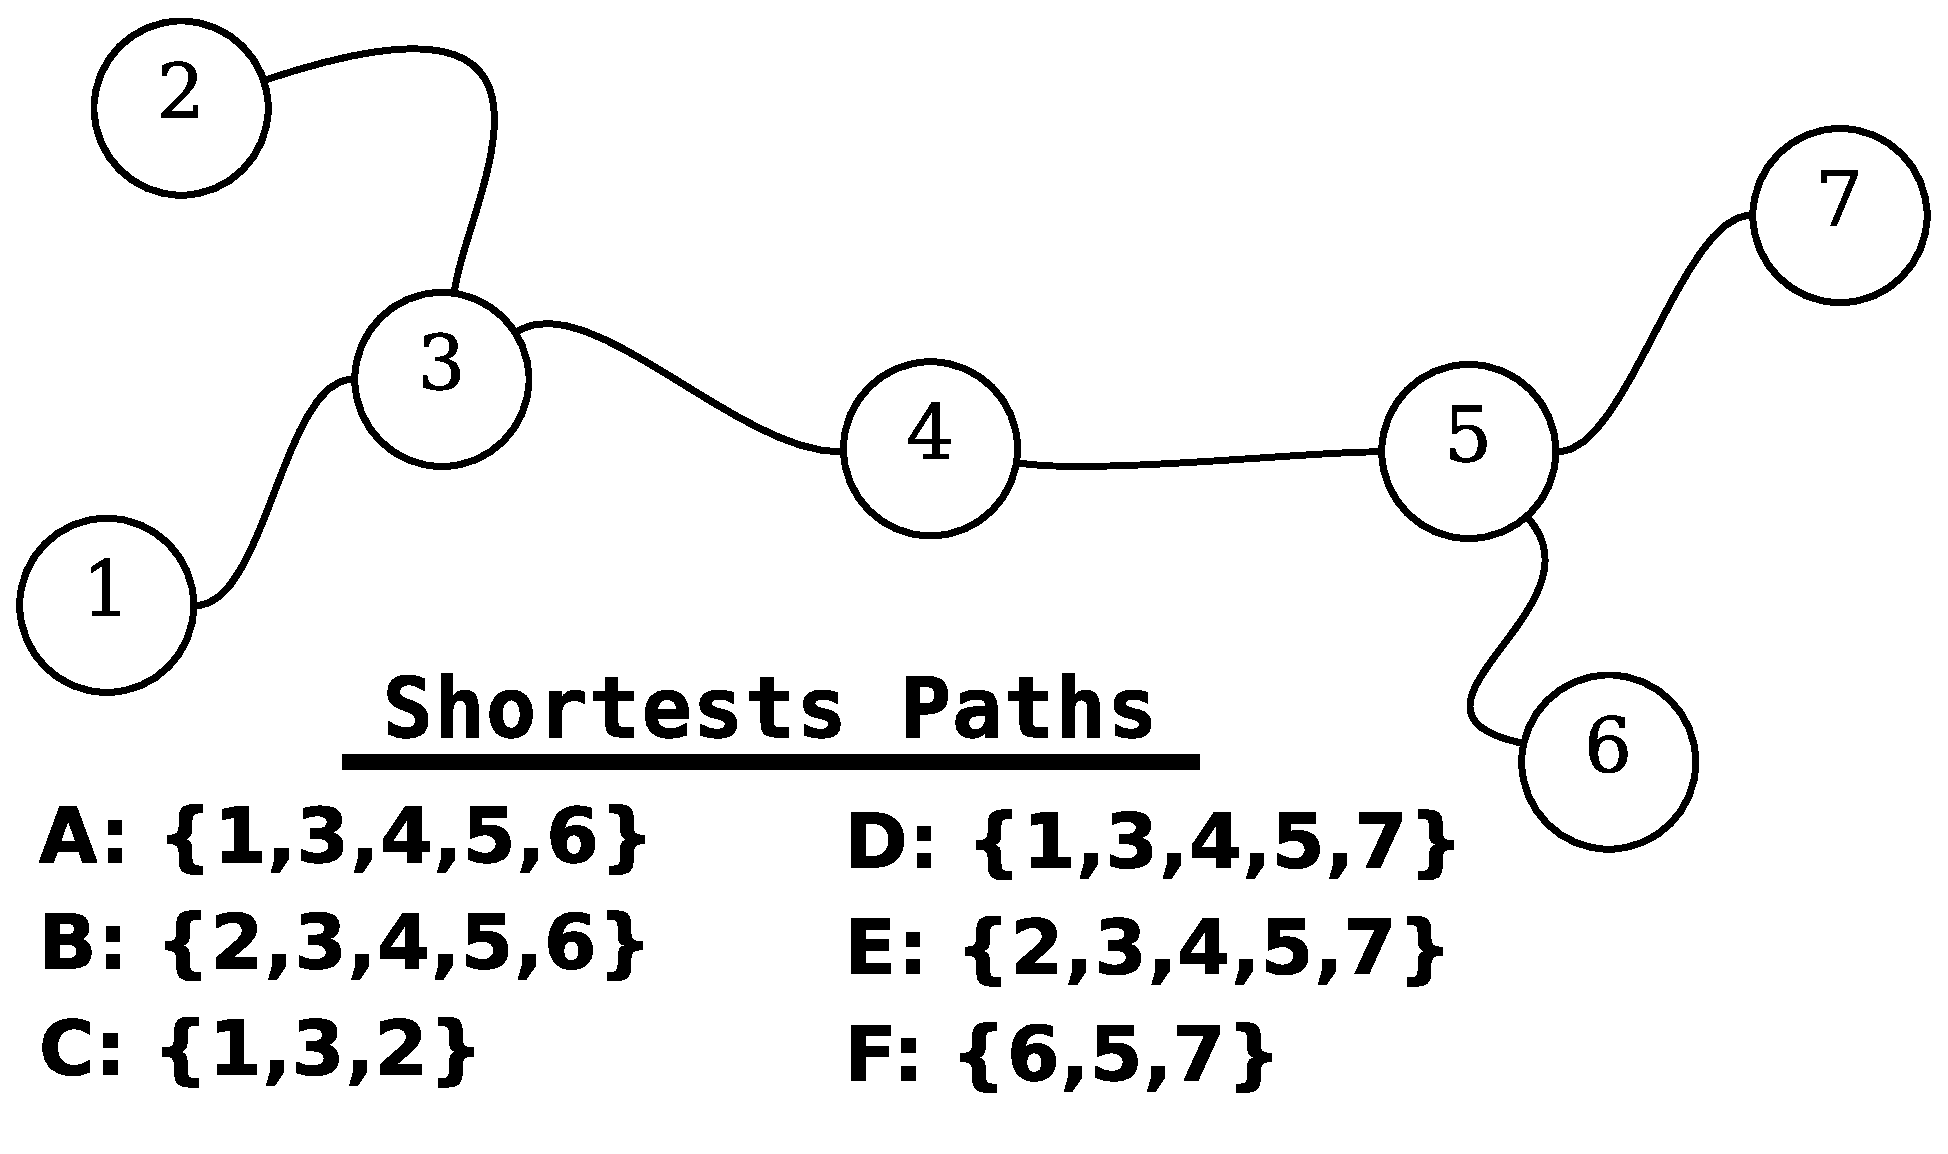
\includegraphics[width=0.4\textwidth]{images/rxmap} 
% 
%     \hspace{-2em}$\gamma(\Psi)=1*2+1*4+3*3=15$\\
% 
%   \begin{exampleblock}{$\gamma(P_{1,6}) + \gamma(P_{3,6}) \neq \gamma(\Psi)$}
% \hspace{0.7em} (15) \hspace{1.8em} (9)
%   \end{exampleblock}
% \end{frame}


\begin{frame}[shrink=5]  %hmm.. thought i could change colour here :S
\frametitle{Cache: SP Result Ranking} 

 Greedy algorithm


{\small
\begin{tabular}{@{}|c@{}|c@{}|@{}}
\hline
Timestamp & Query \\ \hline 
$T_1$ & $Q_{3,6}$ \\ \hline 
$T_2$ & $Q_{1,6}$ \\ \hline 
$T_3$ & $Q_{2,7}$ \\ \hline 
$T_4$ & $Q_{1,4}$ \\ \hline 
$T_5$ & $Q_{4,8}$ \\ \hline 
$T_6$ & $Q_{2,5}$ \\ \hline 
$T_7$ & $Q_{3,6}$ \\ \hline  
$T_8$ & $Q_{3,6}$ \\ \hline 
\end{tabular}
}


  \begin{picture}(0.0,0.0) 
     \put(90,5){  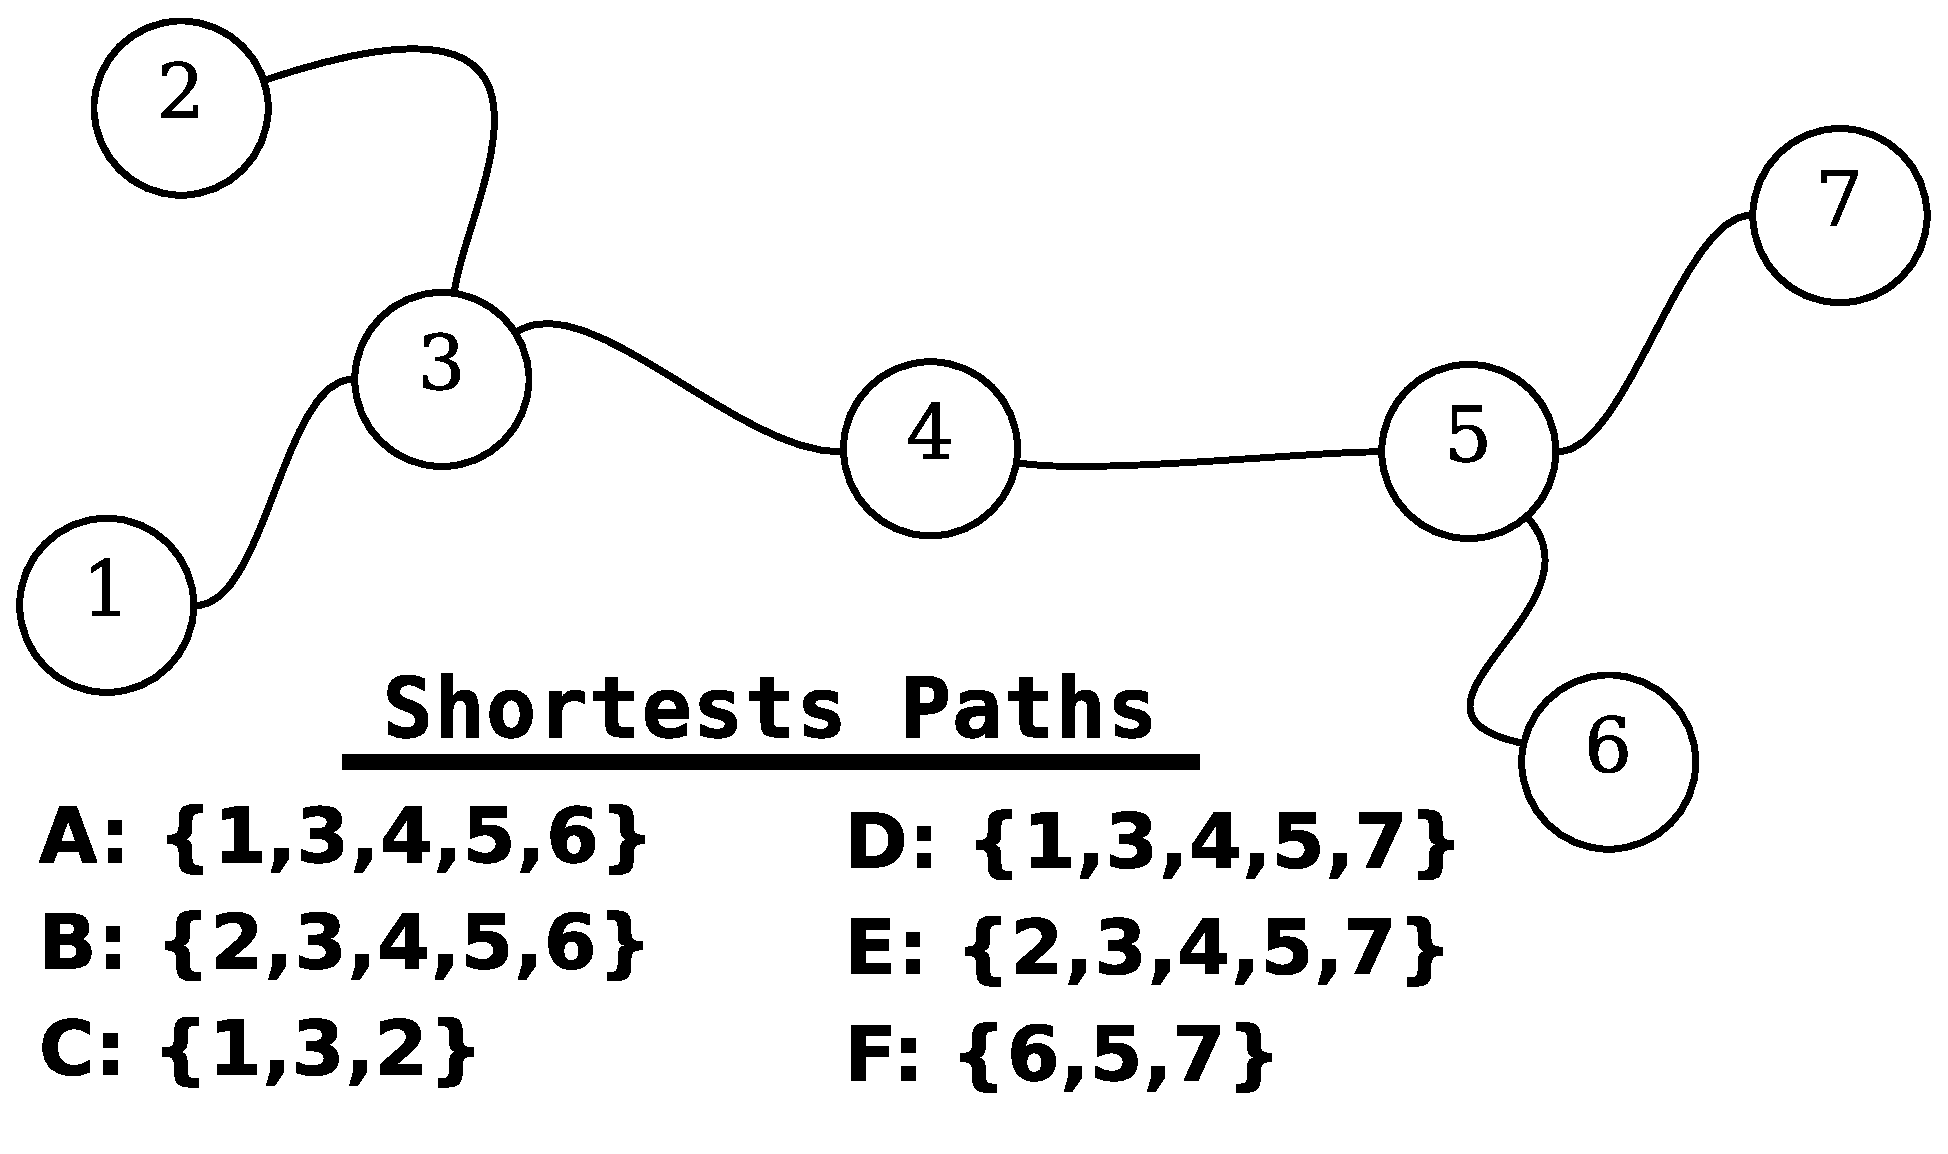
\includegraphics[width=0.7\textwidth]{images/rxmap} }
  \end{picture}



{\small
\begin{tabular}{|c||c|c|c|c|c|c||c|c|}\hline
    Round & \multicolumn{6}{c||}{Path} & \multicolumn{2}{@{ }c@{ }|}{Cache $\Psi$ }  \\ \cline{2-9}
             	& $P_{1,4}$ & $P_{1,6}$ & $P_{2,5}$ & $P_{2,7}$ & $P_{3,6}$ &  $P_{4,8}$ & Before &  After 	 	 \\\hline \hline
    1	&  1/3    & \zebox{\bf 5/5}	 & 1/4    & 2/5 &  3/4    & 1/4 &  empty    & $P_{1,6}$ \\\hline
    2	&      &  &     &  &     &  & $P_{1,6}$    & $P_{1,6}, {\bf ?}$  \\\hline
\end{tabular}
}
\end{frame}


\begin{frame}[shrink=5]  %hmm.. thought i could change colour here :S
\frametitle{Cache: SP Result Ranking - Incremental benefit} 


Incremental benefit calculation



{\small
\begin{tabular}{@{}|c@{}|c@{}|@{}}
\hline
Timestamp & Query \\ \hline 
$T_1$ & $Q_{3,6}$ \\ \hline 
$T_2$ & $Q_{1,6}$ \\ \hline 
$T_3$ & $Q_{2,7}$ \\ \hline 
$T_4$ & $Q_{1,4}$ \\ \hline 
$T_5$ & $Q_{4,8}$ \\ \hline 
$T_6$ & $Q_{2,5}$ \\ \hline 
$T_7$ & $Q_{3,6}$ \\ \hline  
$T_8$ & $Q_{3,6}$ \\ \hline 
\end{tabular}
}


  \begin{picture}(0.0,0.0) 
     \put(90,5){  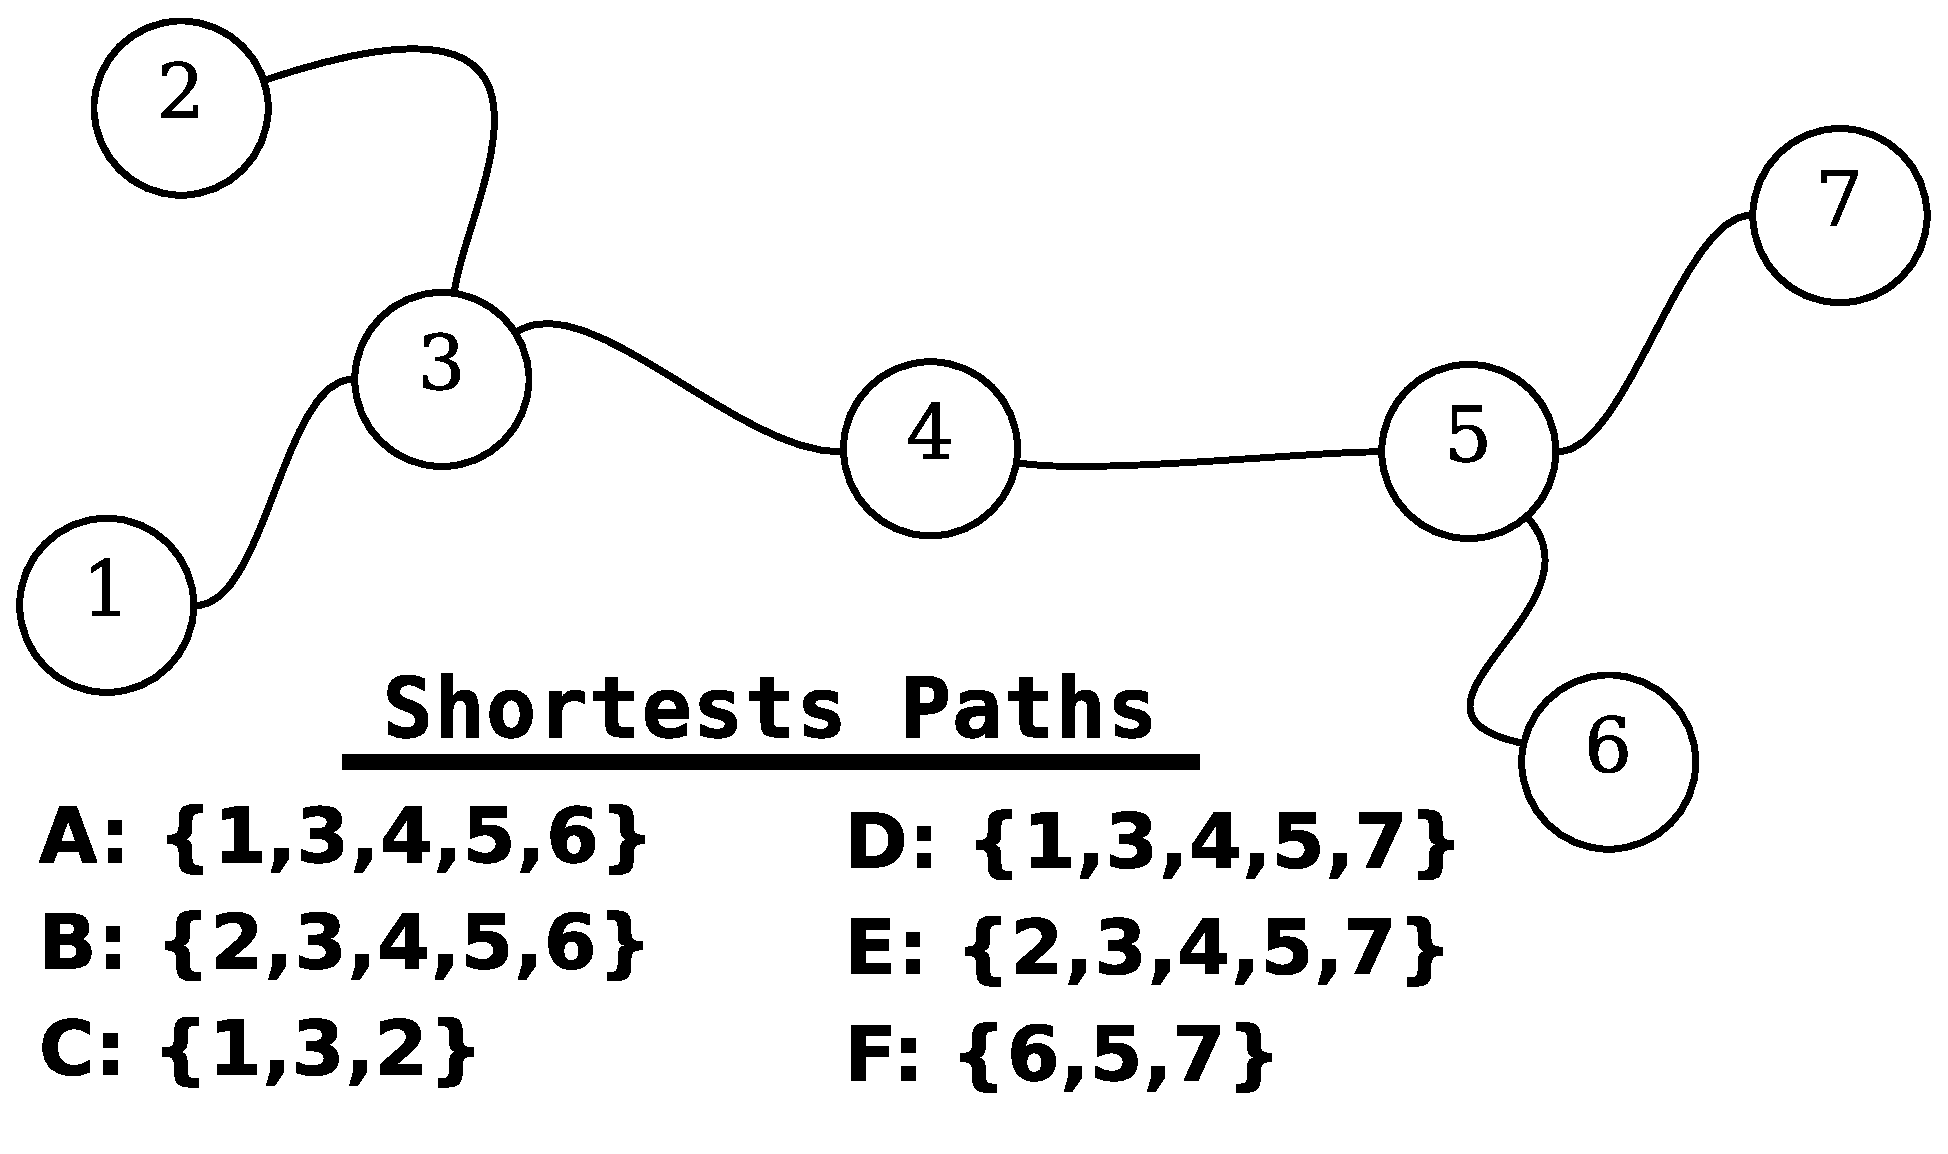
\includegraphics[width=0.7\textwidth]{images/rxmap} }
  \end{picture}



{\small
\begin{tabular}{|c||c|c|c|c|c|c||c|c|}\hline
    Round & \multicolumn{6}{c||}{Path} & \multicolumn{2}{@{ }c@{ }|}{Cache $\Psi$ }  \\ \cline{2-9}
             	& $P_{1,4}$ & $P_{1,6}$ & $P_{2,5}$ & $P_{2,7}$ & $P_{3,6}$ &  $P_{4,8}$ & Before &  After 	 	 \\\hline \hline
    1	&  1/3    & \zebox{\bf 5/5}	 & 1/4    & 2/5 &  3/4    & 1/4 &  empty    & $P_{1,6}$ \\\hline
    2	&  0    & 0 &  1/4    & \zebox{\bf 2/5} &  0    & 1/4 & $P_{1,6}$    & $P_{1,6}, P_{2,7}$  \\\hline
\end{tabular}
}
\end{frame}


\subsection{Data Structure}
\begin{frame}[red] %hmm.. thought i could change colour here :S
\frametitle{Efficient Data Structure for the Cache - Faster lookup} %Maybe a figure to easily explain the main point

\begin{itemize}
\item Lookup time grows with size cache 
\item Support return of full or partial cache items
\end{itemize}

\begin{figure}[hbt]
  \center %\small
  \begin{tabular}{@{}c@{}c@{ }c@{}}
    \begin{tabular}{c|l|}
        \cline{2-2}
        $\Psi_1$ & $v_1, v_3, v_4$ \\ \cline{2-2}
        $\Psi_2$ & $v_1, v_3, v_2$ \\ \cline{2-2}
        $\Psi_3$ & $v_2, v_3, v_4, v_5$ \\ \cline{2-2}
%        $\Psi_4$ & $v_3, v_4, v_5, v_6$ \\ \cline{2-2}
%        $\Psi_5$ & $v_3, v_4, v_5, v_7$ \\ \cline{2-2}
    \end{tabular}
    &
    \begin{tabular}{c|l|}
        \cline{2-2}
        $v_1$ & $\Psi_1, \Psi_2$ \\ \cline{2-2}
        $v_2$ & $\Psi_2, \Psi_3$ \\ \cline{2-2}
        $v_3$ & $\Psi_1, \Psi_2, \Psi_3$ \\ \cline{2-2}
        $v_4$ & $\Psi_1, \Psi_3$ \\ \cline{2-2}
        $v_5$ & $\Psi_3$ \\ \cline{2-2}
    \end{tabular}
  &
    \begin{tabular}{c}
    \\
    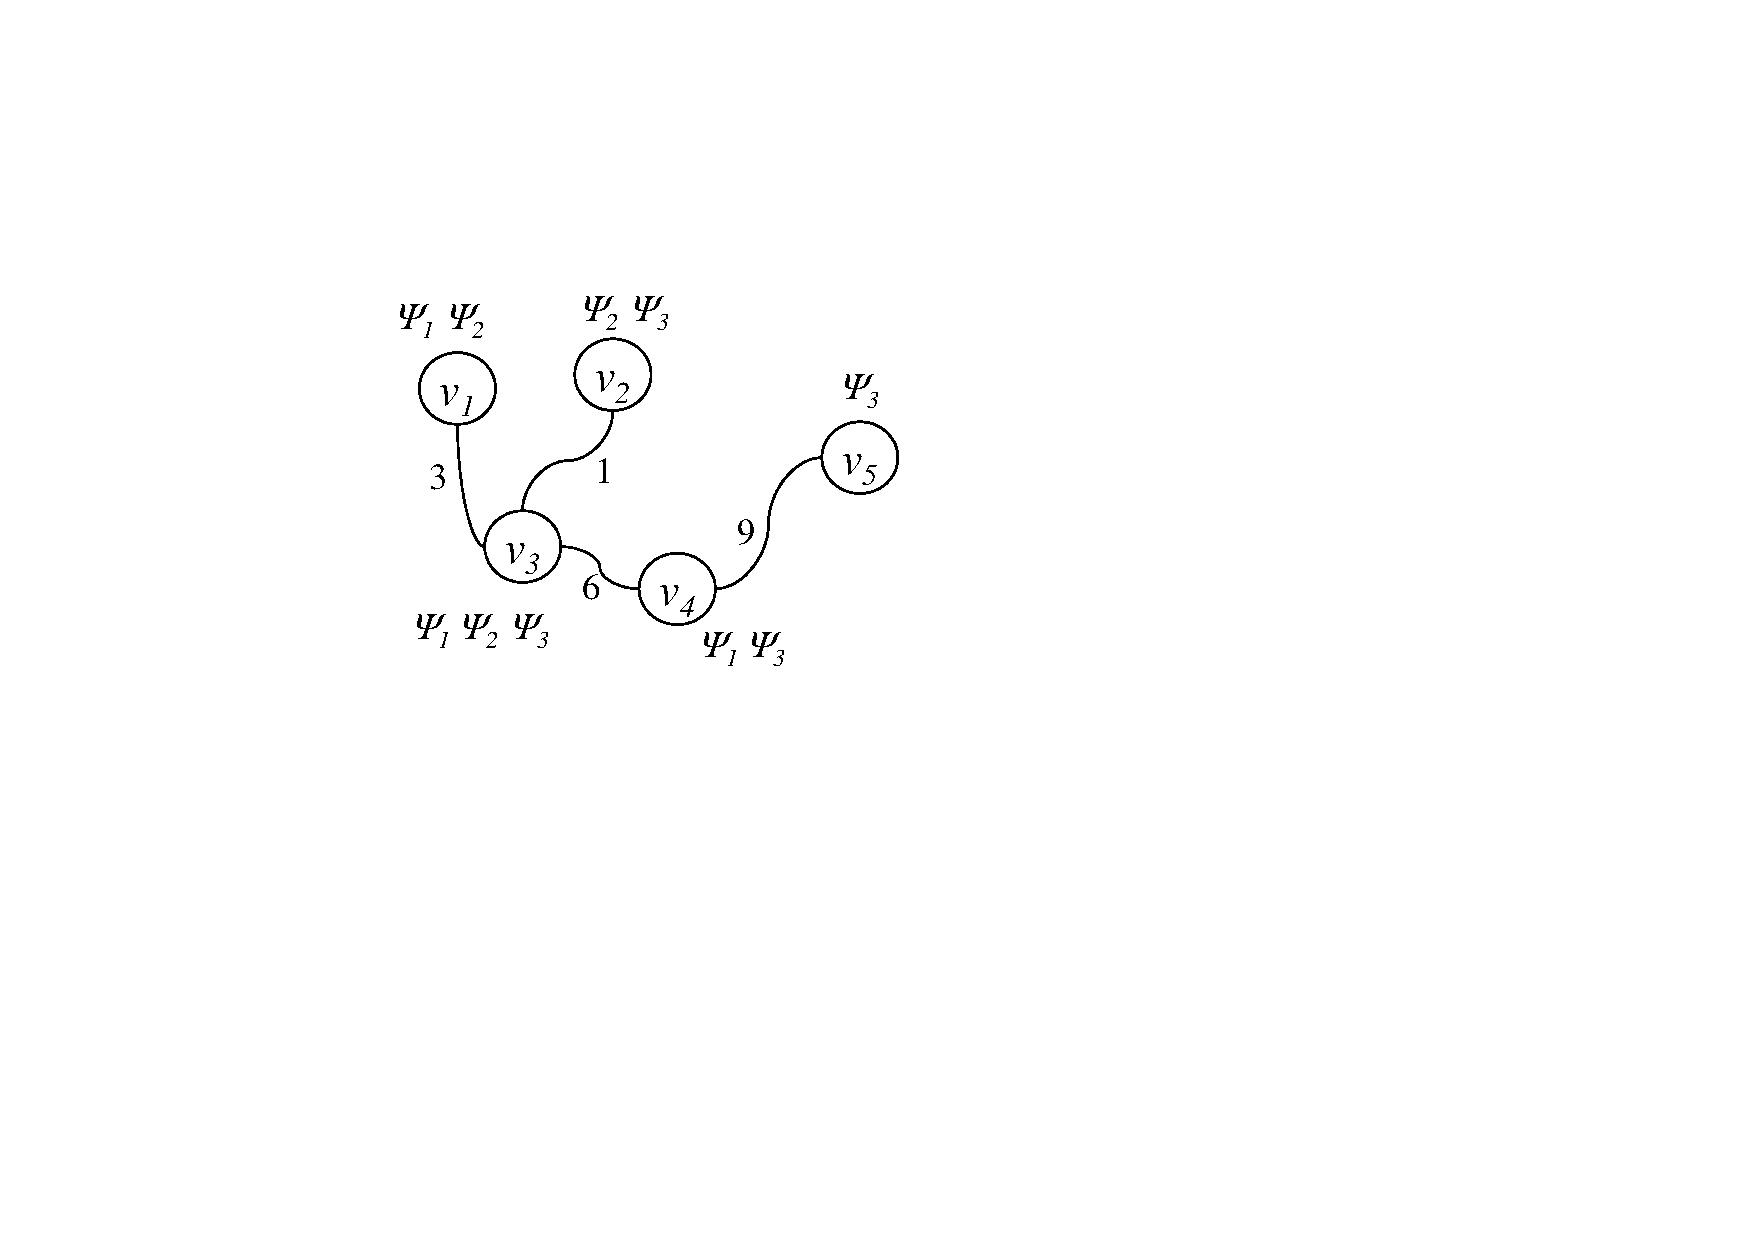
\includegraphics[width=0.4\columnwidth]{images/cachegraph}
    \end{tabular}
    \\
     Paths & \hspace{1.5em} Inverted List & \hspace{1.5em} Visualization
  \end{tabular}
\end{figure}

\end{frame}


\begin{frame}[shrink=10] %hmm.. thought i could change colour here :S
\frametitle{Efficient Data Structure for the Cache - Efficient storage} %Maybe a figure to easily explain the main point

\begin{itemize}
\item Support efficient lookup and return of full or partial cache items\\
\item Compact storage of shortest paths
\end{itemize}
\makebox[\linewidth]{\parbox{14cm}{
\begin{figure}[hbt]
  \center \small \hspace{-2em}
  \begin{tabular}{@{}c@{}c@{ }c@{}}
    \begin{tabular}{c|l|}
	      \multicolumn{2}{c}{} \\\cline{2-2}
        $v_1$ & $v_3$ \\ \cline{2-2}
        $v_2$ & $v_3$ \\ \cline{2-2}
        $v_3$ & $v_1, v_2, v_4$ \\ \cline{2-2}
        $v_4$ & $v_3, v_5$ \\ \cline{2-2}
        $v_5$ & $v_4$ \\ \cline{2-2}
    \end{tabular}
   &
    \begin{tabular}{c|l|c|}
        \multicolumn{3}{c}{~~~~~~content~~~~parent} \\
        \cline{2-3}
        $v_1$ & $\Psi_1, \Psi_2$ & NIL \\ \cline{2-3}
        $v_2$ & $\cdots$ & $\cdots$ \\ \cline{2-3}
        $v_3$ & $\Psi_3$ & $v_1$ \\ \cline{2-3}
        $v_4$ & $\cdots$ & $\cdots$ \\ \cline{2-3}
        $v_5$ & $\cdots$ & $\cdots$ \\ \cline{2-3}
    \end{tabular}
  &
    \begin{tabular}{@{}c@{}}
    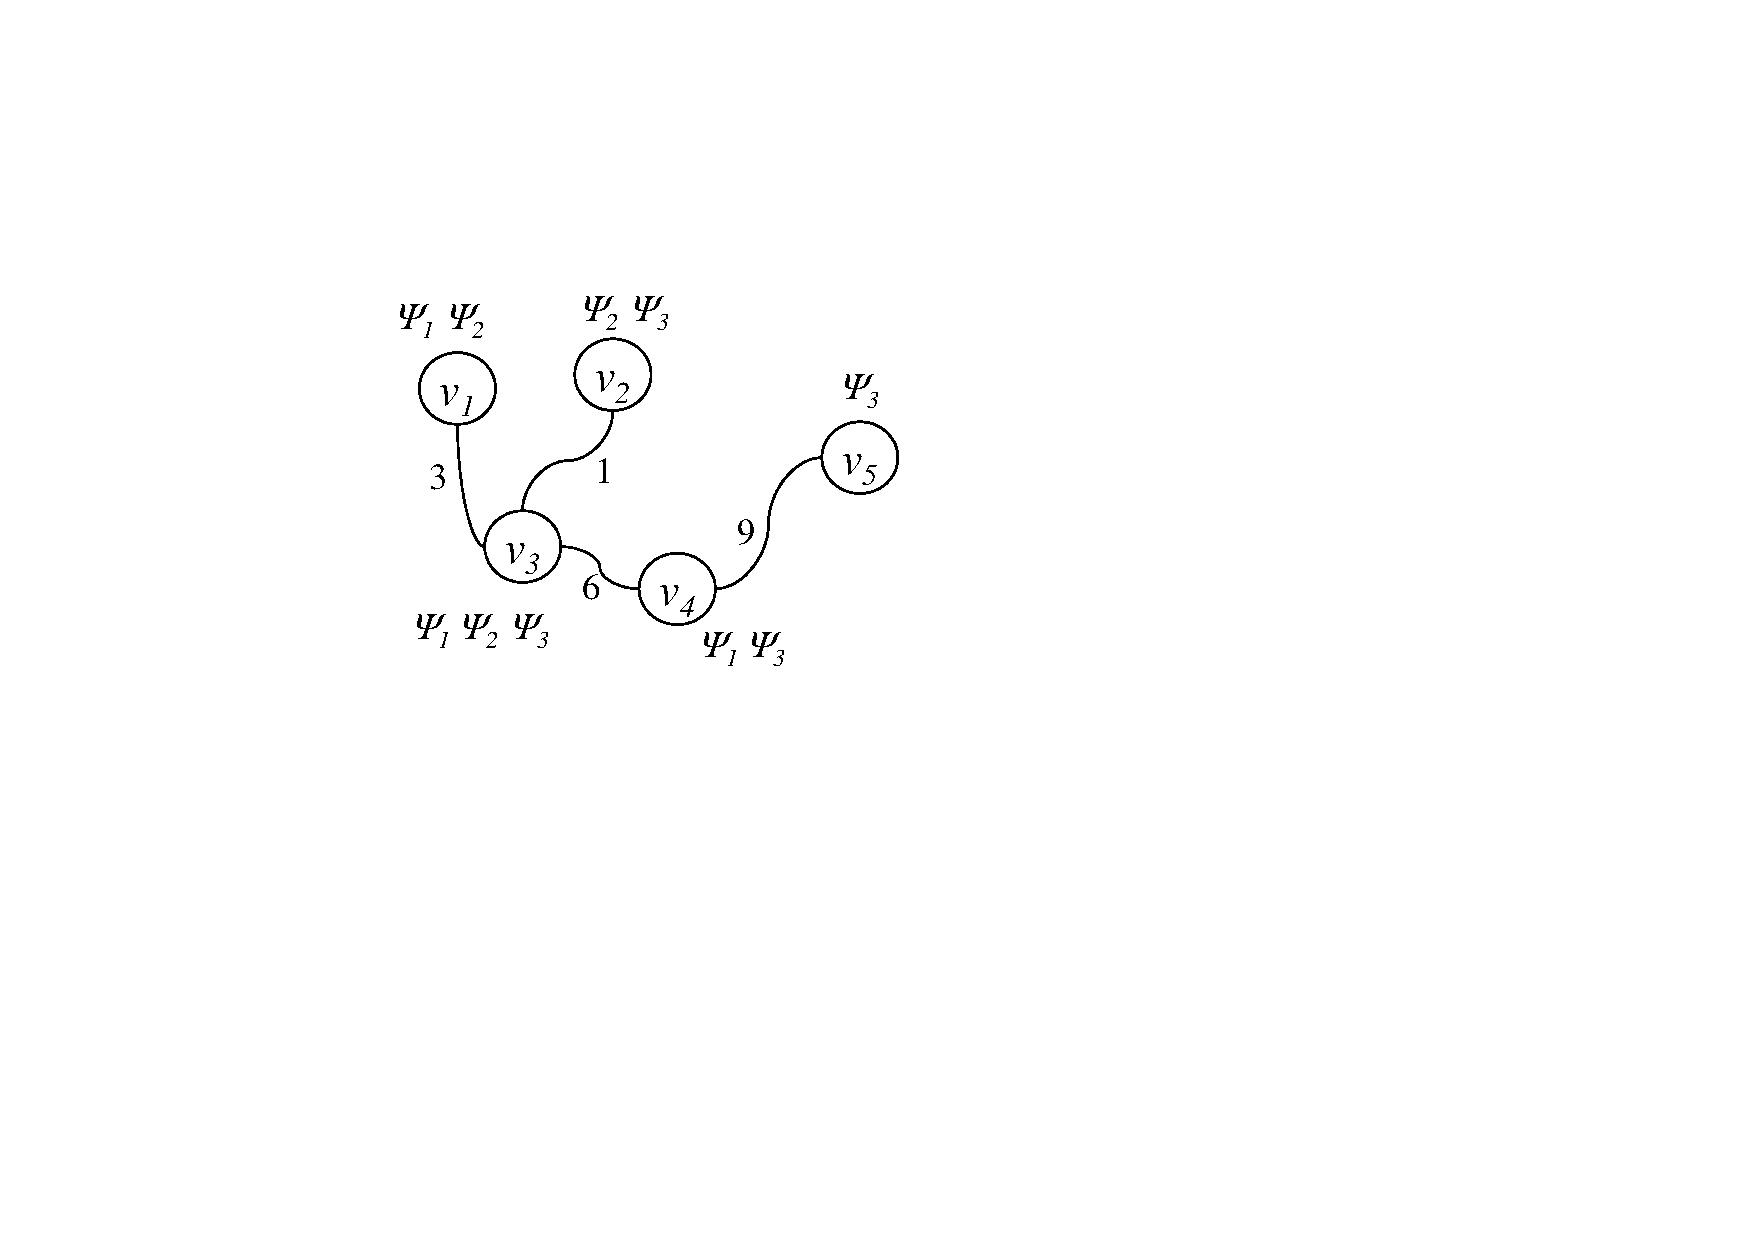
\includegraphics[width=0.45\columnwidth]{images/cachegraph}
    \end{tabular}
    \\
    %\hspace{1.5em}Inverted lists & 
    \hspace{1em}Graph representation &  \hspace{1.5em}Prefix compressed & Visualization
  \end{tabular}
\end{figure}
}}

\end{frame}
